\documentclass{article}
\usepackage{amsmath}
\usepackage[utf8]{inputenc}
\usepackage{graphicx}
\usepackage{verbatim}
\usepackage{float}
\usepackage[makeroom]{cancel}
\usepackage[english]{babel}
\usepackage{textcomp}
\usepackage{gensymb}
\usepackage{color}
\usepackage{subcaption}
\usepackage{caption}
\usepackage{hyperref}
\usepackage{physics}
\usepackage{dsfont}
%\usepackage{amsfonts}
\usepackage{listings}
\usepackage{multicol}
\usepackage{units}

\usepackage[mathscr]{eucal}

% From Eirik's .tex
\usepackage{epstopdf}
\usepackage{cite}
\usepackage{braket}
\usepackage{url}
\bibliographystyle{plain}

\usepackage{algorithmicx}
\usepackage{algorithm}% http://ctan.org/pkg/algorithms
\usepackage{algpseudocode}% http://ctan.org/pkg/algorithmicx

\usepackage[margin=1cm]{caption}
\usepackage[outer=1.2in,inner=1.2in]{geometry}
% For writing full-size pages
%\usepackage{geometry}
%\geometry{
%  left=5mm,
%  right=5mm,
%  top=5mm,
%  bottom=5mm,
%  heightrounded,
%}

% Finding overfull \hbox
\overfullrule=2cm

\lstset{language=IDL}
 %\lstset{alsolanguage=c++}
\lstset{basicstyle=\ttfamily\small}
 %\lstset{backgroundcolor=\color{white}}
\lstset{frame=single}
\lstset{stringstyle=\ttfamily}
\lstset{keywordstyle=\color{red}\bfseries}
\lstset{commentstyle=\itshape\color{blue}}
\lstset{showspaces=false}
\lstset{showstringspaces=false}
\lstset{showtabs=false}
\lstset{breaklines}
\lstset{aboveskip=20pt,belowskip=20pt}

\lstset{basicstyle=\footnotesize, basewidth=0.5em}
\lstdefinestyle{cl}{frame=none,basicstyle=\ttfamily\small}
\lstdefinestyle{pr}{frame=single,basicstyle=\ttfamily\small}
\lstdefinestyle{prt}{frame=none,basicstyle=\ttfamily\small}
% \lstinputlisting[language=Python]{filename}


\definecolor{codepurple}{rgb}{0.58,0,0.82}
\definecolor{backcolour}{rgb}{0.95,0.95,0.92}
\definecolor{dkgreen}{rgb}{0,0.6,0}
\definecolor{gray}{rgb}{0.5,0.5,0.5}
\definecolor{magenta}{rgb}{0.58,0,0.82}

\lstdefinestyle{pystyle}{
  language=Python,
  aboveskip=3mm,
  belowskip=3mm,
  columns=flexible,
  basicstyle={\small\ttfamily},
  backgroundcolor=\color{backcolour},
  commentstyle=\color{dkgreen},
  keywordstyle=\color{magenta},
  numberstyle=\tiny\color{gray},
  stringstyle=\color{codepurple},
  basicstyle=\footnotesize,
  breakatwhitespace=false,
  breaklines=true,
  captionpos=b,
  keepspaces=true,
  numbers=left,
  numbersep=5pt,
  showspaces=false,
  showstringspaces=false,
  showtabs=false,
  tabsize=2
}

%%%%%%%%%%%%%%%%%%%%%%%%%%%%%%%%
% Self made macros here yaaaaaay
\newcommand\answer[1]{\underline{\underline{#1}}}
\newcommand\pd[2]{\frac{\partial #1}{\partial #2}}
\newcommand\red[1]{\textcolor{red}{\textbf{#1}}}
\newcommand\numberthis{\addtocounter{equation}{1}\tag{\theequation}}
% Usage: \numberthis \label{name}
% Referencing: \eqref{name}

% Some matrices
\newcommand\smat[1]{\big(\begin{smallmatrix}#1\end{smallmatrix}\big)}
\newcommand\ppmat[1]{\begin{pmatrix}#1\end{pmatrix}}

%%%%%%%%%%%%%%%%%%%%%%%%%%%%%%%%%
% Eirik's self made macros
\newcommand{\s}{^{*}}
\newcommand{\V}[1]{\mathbf{#1}}
\newcommand{\husk}[1]{\color{red} #1 \color{black}}
\newcommand{\E}[1]{\cdot 10^{#1}}
\newcommand{\e}[1]{\ \text{#1}}
\newcommand{\tom}[1]{\big( #1 \big)}
\newcommand{\Tom}[1]{\Big( #1 \Big)}
\newcommand{\tomH}[1]{\big[ #1 \big] }
\newcommand{\TomH}[1]{\Big[ #1 \Big]}
\newcommand{\tomK}[1]{ \{ #1 \} }
\newcommand{\TomK}[1]{\Big\lbrace #1 \Big\rbrace}
\newcommand{\bigabs}[1]{\left| #1 \right|}

% Section labeling
\usepackage{titlesec}% http://ctan.org/pkg/titlesec
\renewcommand{\thesubsection}{\arabic{subsection}}


% Title/name/date
\title{FYS4150 - Project 4}
\author{Eirik Ramsli Hauge}
\date{16. November 2016}

\begin{document}
\maketitle
\begin{abstract}
The aim of this project is to study the Ising model using the Metropolis algorithm and Monte Carlo cycles where one cycle is one runthrough through the Metropolis algorithm. We will mostly change the variables spin lattice size L$^2$ and temperature to aquire our results. First we will compare our analytical expression to a numerical for a 2x2 case. Then we will expand to a 20x20 case. We will also look at the number of accepted spin flips after all cycles for differen temperatures and find the probaility of finding an energy as a function of two temperatures and look at variance. \\
Lastly we will use parallelization and look at many temperatures with increasing L and find the critical temperature. \\ \\
We found that there was a good agrement between our analytical and numerical expression. The number of accepted states increased rapidly with T, the probability plots made sense, the variance did not and our critical temperatures came closer and closer to the limit found by Onsager with increasing L.
\end{abstract}
\subsection*{Introduction}
Phase transitions is ofthe thought of as a transition between liquid and vaport or solids. This however is not always the case. We can also have magnetic transitions and a popular model to study this is the Ising model. This model studies the phase transition between a magnetic phase and a phase with zero magnetization. To simplify our problem, we will look at a two dimensional system without an external magnetic field. We will mostly look at the values for $\langle E \rangle$, $\langle M \rangle$ $C_v$ and $\chi$ as a function of T.\\ \\
First of all we will study the 2x2 case analytically, develop a code based on the Ising model and the metropolis algorithm and compare the numerical values with the analytical ones. The metropolis algorithm will always try to diminish the Energy of the system so that we reach the stabil state.\\
When we know our code is working we will increase to a 20x20 lattice and find how many Monte Carlo cycles are needed before the different eigenvalues reach an equilibrium for different temperatures. We will also look at how many times we flip a spin to across all Monte Carlo cycles. \husk{Er det dette vi gjør?} \\
Afterwards we will look at the probability $P(E)$ of finding an energy after equilibrium is reached by counting each energy we find. \\ \\
Lastly we will use parallelization to calculate larger with L-values for many values of T. To do this we will use MPI. The results will be analyzed and used to find the critical temperature $T_C$ in the thermodynamical limit $L \rightarrow \infty$. \\ \\
There are several good reason for why we are doing this experiment as a lesson in Computational Physics. By using the Ising model and the metropolis algorithm over many cycles we get a good insight into Monte Carlo calculations and by using MPI we learn about paralellization and the benefits of being able to use every core at once. These tricks teaches us that it's allowed to think before you code, which is always a good thing.
\subsection*{Theory}
The Ising model's total energy for a $L$ x $L$  spin lattice in state $i$ can in it's simplest form be expressed as follows:
\begin{equation}
E_i = - J \sum\limits_{\langle kl \rangle}^N s_k s_l - \mathcal{B}\sum \limits_{k}^N s_k
\label{eq:Etot}
\end{equation}
Where $J$ is a coupling constant expressing the strength of the interaction between neighboring spins. The $\langle kl \rangle$ expresses that we only wish to look at neighboring spins, $s = \pm 1$, $N$ is the number of spin states and $\mathcal{B}$ is an external magnetic field which will be set to 0 in this experiment. \\ \\
To calculate the wanted expectation values $\langle E \rangle$ and $\langle |M| \rangle$ we have the expressions:
\begin{equation}
\langle E \rangle = \sum \limits_i E_i P_i(\beta)
\label{eq:Eexp}
\end{equation} 
and 
\begin{equation}
\langle |M| \rangle = \sum \limits_i |M_i| P_i(\beta)
\label{eq:Mexp}
\end{equation}
$E_i$ and $M_i$ are respectively the energy (equation \eqref{eq:Etot}) and the magnetization in the state $i$. The magnetization is given as:
\begin{equation}
M_i = \sum \limits_k^N s_k
\label{eq:Mtot}
\end{equation} 
$P_i(\beta)$ is the probability distribution for the state $i$ and is given as:
\begin{equation}
P_i(\beta) = \frac{e^{-\beta E_i}}{Z}
\label{eq:probdist}
\end{equation}
where $\beta = 1/(k_B T)$ where $k_B$ is the Boltzmann constant and $T$ is the temperature. and $Z$ is the partition function given as:
\begin{equation}
Z = \sum \limits_{i = 1}^M e^{- \beta E_i}
\label{eq:distribution}
\end{equation}
When all the above equations are known, it is easy to find the heat capacity $C_v$ and susceptibility $\chi$:
\begin{equation}
C_v = \frac{\sigma_E^2}{k_B T^2} = \frac{\langle E^2 \rangle - \langle E \rangle ^2}{k_B T^2}
\label{eq:heatc}
\end{equation}
\begin{equation}
\chi = \frac{\sigma_M^2}{k_B T} = \frac{\langle M^2 \rangle - \langle |M| \rangle ^2}{k_B T}
\label{eq:suscept}
\end{equation}
where for any discrete variable A $\sigma_A^2$ is called the variance of A and
\begin{equation}
\langle A^2 \rangle = \sum_i A_i^2 P_i(\beta)
\label{eq:var}
\end{equation}
all other variables are as above.
\subsubsection*{The 2x2 case}
If we have a lattice with 2x2 spins, there are 16 different spin configurations possible:
\begin{table}[H]
\centering
\caption{Possible spin configurations (degeneracy): All spins up (1), one spin down (4), two spins down side by side (4), two spins down diagonally (2), three spins down (4), all spins down (1).}
\begin{tabular}{c c}
$\uparrow$ & $\uparrow$ \\
$\uparrow$ & $\uparrow$
\end{tabular} \quad
\begin{tabular}{c c}
$\downarrow$ & $\uparrow$ \\
$\uparrow$ & $\uparrow$
\end{tabular}
$\cdots$
\begin{tabular}{c c}
$\downarrow$ & $\downarrow$ \\
$\uparrow$ & $\uparrow$
\end{tabular}
$\cdots$
\begin{tabular}{c c}
$\uparrow$ & $\downarrow$ \\
$\downarrow$ & $\uparrow$
\end{tabular}
\quad
\begin{tabular}{c c}
$\downarrow$ & $\uparrow$ \\
$\uparrow$ & $\downarrow$ 
\end{tabular}
$\cdots$
\begin{tabular}{c c}
$\downarrow$ & $\uparrow$ \\
$\downarrow$ & $\downarrow$
\end{tabular}
\quad
\begin{tabular}{c c}
$\downarrow$ & $\downarrow$ \\
$\downarrow$ & $\downarrow$
\end{tabular}
\label{tab:spinconfiguration}
\end{table}
The properties of the different spin states illustrated in table \ref{tab:spinconfiguration} are better expressed in table \ref{tab:spinvalues}
\begin{table}[H]
\centering
\caption{Energy, magnetization and degeneracy as a function of number of spins up for a 2 x 2 lattice. Energy and magnetization calculated by equation \eqref{eq:Etot} and \eqref{eq:Mtot}}
\begin{tabular}{c|c|c|c c}
Number of spins up & Degeneracy & Energy & M \\ \cline{1-4}
4 & 1 & $-8 J$ & 4 \\
3 & 4 & 0 & 2 \\
2 & 4 & 0 & 0 & (side by side) \\
2 & 2 & $8J$ & 0 & (diagonal) \\
1 & 4 & 0 & -2 \\
0 & 1 & $-8J$ & -4
\end{tabular}
\label{tab:spinvalues}
\end{table}
By using equation \eqref{eq:distribution} we find the distributin function:
\begin{align*}
Z &= e^{\beta 8J} + 2e^{-\beta 8J} + e^{\beta 8J} + 12 \cdot e^0 \\
&= 2e^{\beta 8J} + 2e^{-\beta 8J} + 12
\intertext{And then by using equations \eqref{eq:Eexp}, \eqref{eq:Mexp}, \eqref{eq:heatc} and \eqref{eq:suscept} we can easily find respectively $\langle E \rangle$, $\langle |M| \rangle$, $C_v$ and $\chi$}
\langle E \rangle &= \frac{1}{Z} \sum \limits_i^{16} = E_i e^{- \beta E_i} \\
&= \frac{1}{Z} \tomH{-8J e^{\beta 8 J} + 2 \cdot 8J e^{-\beta 8 J} - 8J e^{\beta 8 J}} = -\frac{1}{Z} \tomH{16 J e^{\beta 8 J} - 16 J e^{-\beta 8 J}} \\
&=  -\frac{32 J}{Z} \sinh(\beta 8 J) \\
\langle |M| \rangle &= \frac{1}{Z} \sum \limits_i^{16} = |M_i| e^{- \beta E_i} \\
&= \frac{1}{Z} \tomH{4 e^{\beta 8 J} + 4 \cdot 2 e^0 + 4 \cdot 2 e^0 + 4 e^{\beta 8 J}} = \frac{1}{Z} \tomH{8e^{\beta 8 J} + 16} \\
\langle E^2 \rangle &= \frac{1}{Z} \sum \limits_i^{16} = E_i^2 e^{- \beta E_i}  
= \frac{128 J^2}{Z} \tomH{e^{\beta 8 J} + e^{-\beta 8 J}} 
= \frac{256 J^2}{Z} \cosh(\beta 8 J) \\
\langle M^2 \rangle &= \frac{1}{Z} \sum \limits_i^{16} = M_i^2 e^{- \beta E_i} 
= \frac{32}{Z}(e^{\beta 8 J} + 1) \\
C_v &= \frac{1}{k_B T^2} \TomH{\frac{256 J^2}{Z} \cosh(\beta 8 J) - (- \frac{32 J}{Z} \sinh(\beta 8 J))^2} \\
\chi &= \frac{1}{k_B T} \TomH{\frac{32}{Z}(e^{\beta 8 J} + 1)  - (\frac{1}{Z} \tomH{8e^{\beta 8 J} + 16})^2}
\end{align*} \\
Why is the 2x2 case relevant? There are two good reason: \\
1. It is good to have an analytical example to compare with. \\
2. It gives an easy understandig periodic boundary conditions. Periodic boundary conditions meens that the spin lattice can be looked upon as a 3D torus folded out where if we walk over the edge of the 2D lattice, we end up at the other side. This is an easy consept to grasp if you have played video games like Chrono Trigger where the map functions in the same way. In our 2x2 example this means that the top most left corner will "see" the bottom left spin both above and belove itself. And likewise it will see the top most right spin both to its right and to its left.
\subsubsection*{The Metropolis Algorithm}
Through this project we wish to start with a spin lattice where all spin are known. Then we wish to achieve the stable state, e.i. the state with the lowest energy. To do this we will use both Monte Carlo and the Metropolis algorithm. The Metropolis Algorithm bases itself upon a pretty simple principle and applied to the Ising model it goes like this: \\
\begin{algorithm}[H]
\small
\caption{Metropolis for the Ising Model}\label{alg:Metropolis}
\begin{algorithmic}[1]
\State Initialize a state spin lattice with energy $E_0$ and magnetization $M_0$ 
\For {$i = 0 \rightarrow i = L$}
\For {$j = 0 \rightarrow j = L$} \Comment{we loop over $L^2$ giving all spins a chance to be picked.}
\State Choose random spin $s_{l,k}$
\State Find the difference in energy ($\Delta E$) if we had flipped that spin.
\If{$r \leq e^{-\beta \Delta E}$} \Comment{where r is a random number between 0 and 1.}
\State Flip spin
\State M += 2 $\cdot s_{l,k}$
\State E += $\Delta E$
\EndIf
\EndFor
\EndFor
\State Update Eigenvalues
\end{algorithmic}
\end{algorithm}
By first initializing a spin lattice and then running the Metropolis algorithm many times using the previous spin lattice as the initial state we do a Monte Carlo simulation where each run of the Metropolis is one cycle. \\
For a more in-depth study of the Metropolis Algorithm in general you may read in the Lecture Notes and especially note figure 12.7 as this gives a good overview. \cite{lectures}
\subsubsection*{Stabilization and probability}
The reason we wish to run the Metropolis algorithm many times is to reach the steady state. While the steady state is hard to guess, we will reach it bit by bit by reducing the energy. As one can see from algorithm \ref{alg:Metropolis} we only accept a flip spin if $r \leq e^{-\beta \Delta E}$. As $\beta > 0$ there will be a bigger chance for the negative $\Delta E$ values to cause a spin flip and thus cause a lower overall energy. \\ \\
Once this steady state is reached we can look at the probability of finding a given energy. This is done by simply counting how often a given energy appears and then dividing by the total number of energies.
\subsubsection*{Estimate the Critical Value}
Onsager found that for $L \rightarrow \infty$ the critical temperature was $T_C \simeq 2.269$. In our case we have the function:
\begin{equation}
T_C(L) - T_C(L = \infty) = aL^{-1/v} = a/L
\end{equation}
we are given that v = 1. a is a constant. \\
Numerically we do this by finding the peak of $C_V$ and $\chi$ as a function of T since this is the phase transition between non-zero magnetization and then zero magnetication. This is caused by L. The finding of the peak is the estimation.
\subsection*{Experimental}
The programs used in this project can be found in the GitHub repository \cite{github} in the \texttt{/src/} folder. When running the program, it takes five command line arguments: \texttt{task}, spin lattice size \texttt{L}, \texttt{Monte Carlo cycles}, \texttt{T} which is either \texttt{temperature} or \texttt{Number of temperatures} depending on task and \texttt{spin direction}. The latter is optional and can be set to either \texttt{up}, \texttt{rand} or \texttt{down} which respectively intializes the spin lattice with all spins up, all spins randomly either up or down or all spins down. By default it is set to \texttt{up}. \\
All files containing data will be stored in GitHub under \texttt{/benchmarks/} with a separate subfolder for each task. The program has four different run modes, which will be discussed in more detail below. Many of the run modes are fairly similar, but with some small changes. To make the program more versatile \texttt{L} and \texttt{T} are optional for all \texttt{task} even though the text \cite{Project} ask us to run for specific values in each task.
\subsubsection*{Parallelization}
This program uses \texttt{MPI} for programming. When running the program one should write: \\ 
\texttt{-n} \texttt{(Number of cores to use)} \texttt{Filename} \texttt{task} \texttt{L (Monte Carlo cycles) T (spin direction)} \\
where everything within a paranthesis describes one argument. \\
Although every task can be run with MPI, it is only task e) that is meant to. We therefore recommend setting number of cores to use to one when running all the other tasks.
\subsubsection*{Task b)}
Setting \texttt{task} to \texttt{b} runs the part of the program which is meant to solve task b. Here the text would have us set L = 2, but we have left this optional. For this task \texttt{T} is \texttt{temperature} and should be set to 1.0. All the data is written to: \\
\texttt{eigenvalues\_MC<Monte Carlo cycles>\_dim<L>\_dir<spin direction>\_T<temperature>.txt}  \\
where \texttt{<a>} means the value of a.
\subsubsection*{Task c)}
Setting \texttt{task} to \texttt{c} runs the part of the program which is meant to solve task c. \texttt{L} should be set to 20. The Metropolis algorithm for this part of the program is the same as above. \texttt{T} should be set to either 1.0 or 2.4. All the data is written to: \\
\texttt{eigenvalues\_MC<Monte Carlo cycles>\_dim<L>\_dir<spin direction>\_T<temperature>.txt} 
\subsubsection*{Task d)}
Setting \texttt{task} to \texttt{d} runs the part of the program which is meant to solve task d. \texttt{L} must be set to 20. The reason why \texttt{L} is fixed here is that we have som threshold values for when the system is in a steady state, as this is affected by the size of the spin lattice. Failing to set \texttt{L} to 20 will make the program stop. The Metropolis algorithm for this part of the program is the same as for \texttt{c}, but when we update the eigenvalues we also store the energy if the number of Monte Carlo cycles are above a threshold. Then the program counts how many times every energy is achieved. \texttt{T} is once again temperature and should be set to either 1.0 or 2.4 and \texttt{Monte Caro cycles} should be set to 1000000 for the threshold values to be right. The eigenvalues for each Monte Carlo cycles are written to \\
\texttt{eigenvalues\_MC<Monte Carlo cycles>\_dim<L>\_dir<spin direction>\_T<temperature>.txt}  \\
And all the energies and their counters are written to: \\
\texttt{EnergyValues\_T<temperature>\_dim<L>\_dir<spin direction>.txt}
\subsubsection*{Task e)}
Setting \texttt{task} to \texttt{e} runs the part of the program which is meant to solve task e. \texttt{L} is optional. \texttt{T} sets the number of temperatures in an array from 2.0 to 2.3. The difference between two values in this array, the $dt$, must be less than or equal to 0.05 or else the program will stop. \\
This part of the program is also specially designed to use \texttt{MPI} for paralellizing and by giving each core a specific temperature to work with we can solve for all the temperatures more efficiently. Since we are only interested in the last eigenvalues we do not write to file for each cycle, but only when all the Monte Carlo cycles have been run through for every core with its temperature.

\subsection*{Results}
All runs were performed with 1 000 000 Monte Carlo cycles.
\subsubsection*{L = 2}
Running the program for \texttt{task} b with L = 2, 1 core and T = 1.0 gave us the results in table \ref{tab:taskb}:
\begin{table}[H]
\centering
\caption{Values returned from the program as a function of Monte Carlo Cycles. The first row of variables is from our analytical calculations.}
\begin{tabular}{c|c|c|c|c}
 Monte Carlo cycles & $<E>$ & $<|M|> $& $\sigma_E^2$ & $\sigma_M^2$ \\ \hline
Analytical &-1.99598 & 0.99866 & 0.03208 & 0.00401 \\
100     &-1.86000    & 0.94000 & 1.04160 & 0.20560 \\
1000    &-1.98400    & 0.99350 & 0.12698 & 0.02283 \\
10000   &-1.99440    & 0.99820 & 0.04467 & 0.00519 \\
100000  & -1.99556   & 0.99848 & 0.03544 & 0.00464 \\
1000000 &-1.99572    & 0.99857 & 0.03418 & 0.00428 
\end{tabular}
\label{tab:taskb}
\end{table}
\subsubsection*{L = 20}
Setting L = 20, T = 1.0 or 2.4 and running \texttt{task} c for 1 core gave us the following results:
\begin{figure}[H]
\centering
\begin{subfigure}{0.49 \textwidth}
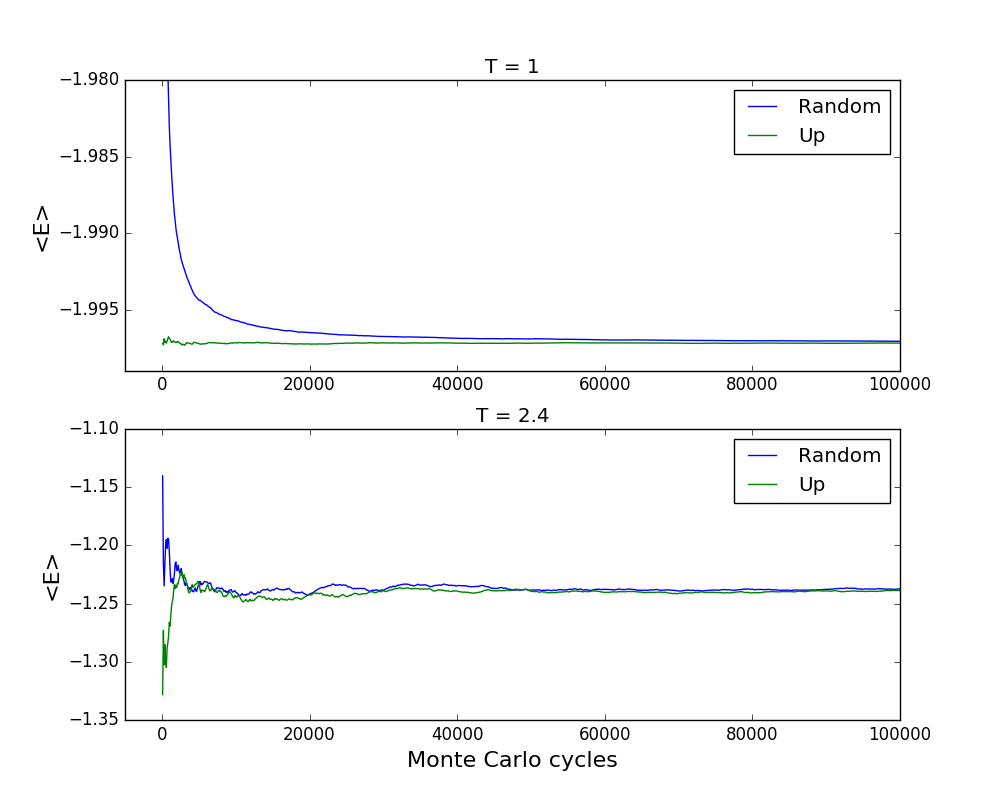
\includegraphics[scale=0.29]{../figures/task_c/energyeig.png}
\label{fig:cEeig}
\end{subfigure}
\begin{subfigure}{0.49 \textwidth}
\centering
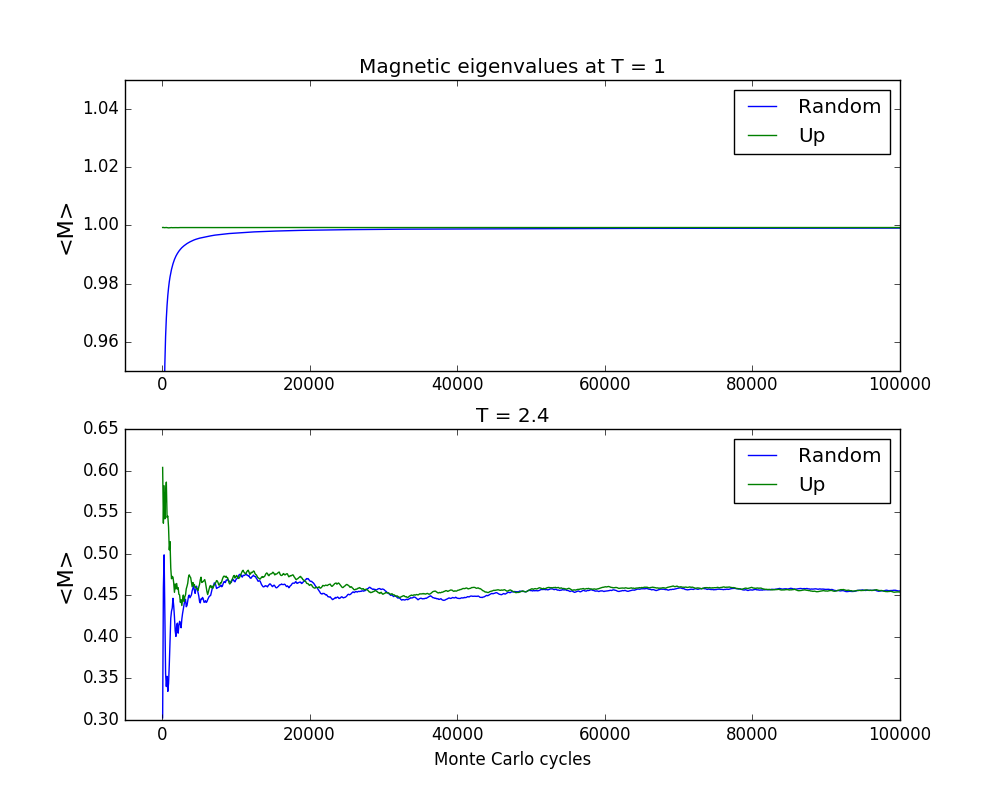
\includegraphics[scale=0.29]{../figures/task_c/Mageig.png}
\label{fig:cMeig}
\end{subfigure}
\caption{Energy and Magnetic eigenvalues as a function of Monte Carlo Cycles for different temperatures. One of the graphs represents the case with all spins fixed upwards. The other representes the case with all spins randomly directed.}
\label{fig:c}
\end{figure}
We can note from figures \ref{fig:c} that there seems to be an equilibrium around 80 000 Monte Carlo cycles for T = 1.0 and around 60 000 for T = 2.4. \\
By looking at the total number of accepted states at the end of all Monte Carlo Cycles as a function of different temperatures we found the correlation shown in figure \ref{fig:cAcc}:
\begin{figure}[H]
\centering
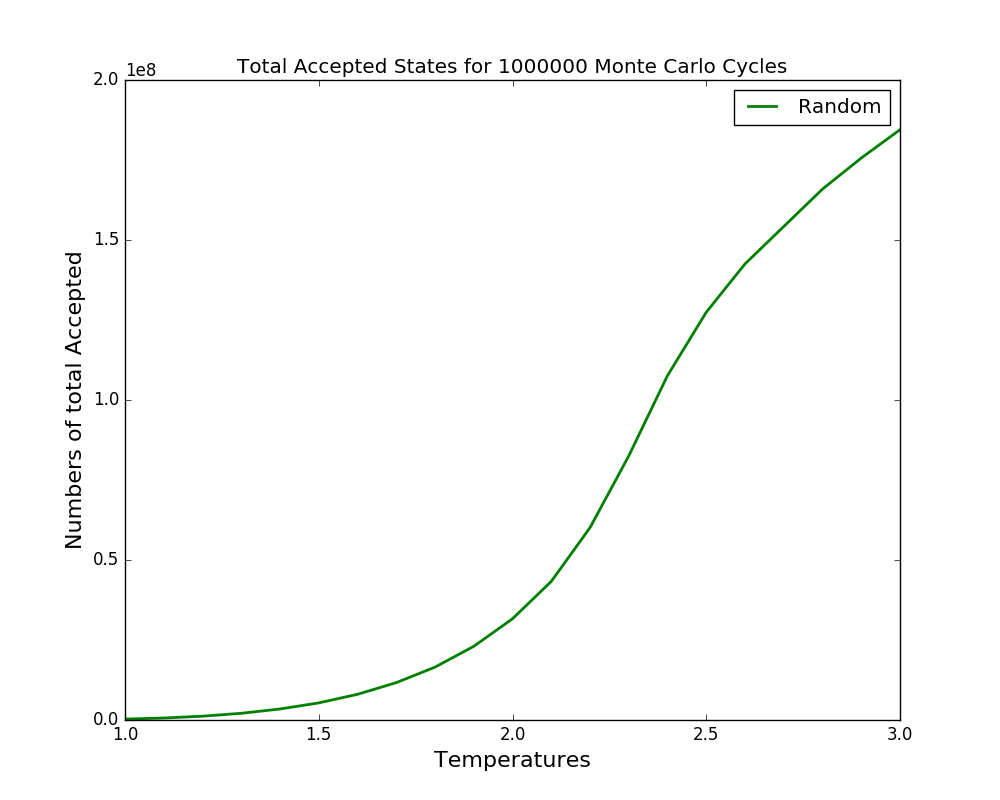
\includegraphics[scale=0.3]{../figures/task_c/accepted.png}
\caption{Number of accepted states after all Monte Carlo cycles as a function of temperature. With L = 2}
\label{fig:cAcc}
\end{figure}
By counting each energy for T = 1.0 and T = 2.4 we found the probabilities shown in figure \ref{fig:cProb}
\begin{figure}[H]
\centering
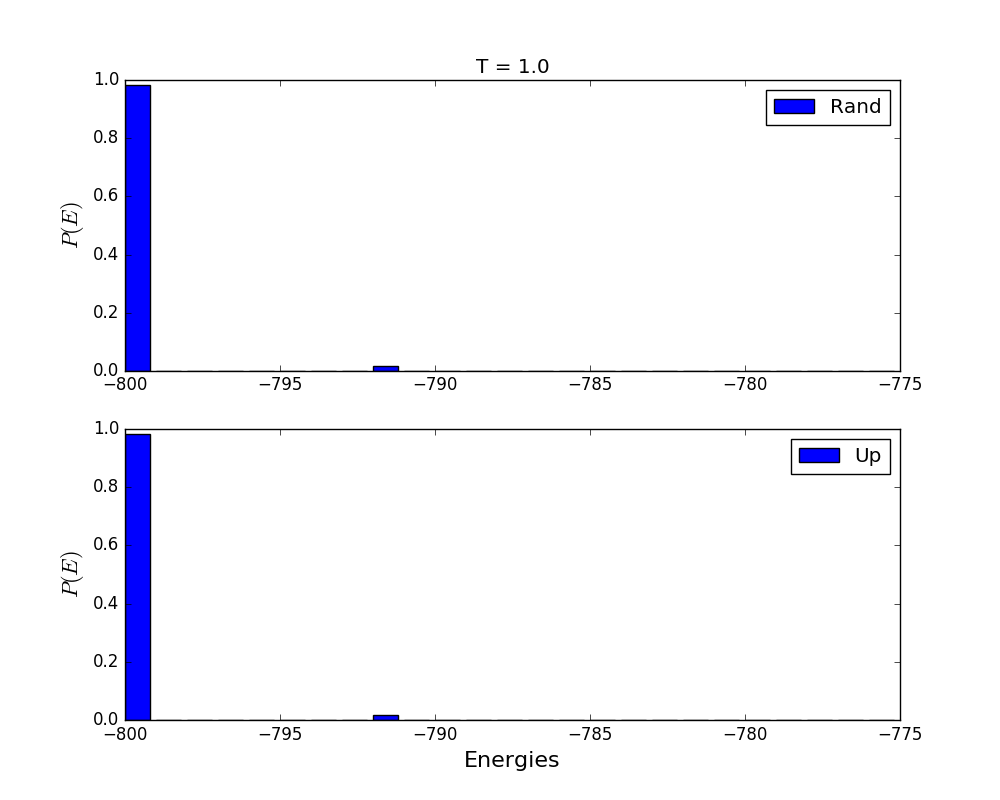
\includegraphics[scale=0.5]{../figures/task_d/hist1.png}
\caption{Probabilities for different energy values for T = 1.0 and T = 2.4. All spins were sett to be initialized randomly.}
\label{fig:cProb}
\end{figure}
By taking the variance of our energies with \texttt{np.var()} and comparing to the last value of $sigma_E^2$ gave us the following presented in table \ref{tab:var}
\begin{table}[H]
\centering
\caption{Variance given directly from the program compared to taking the variance of our energies. As we can see, they are quite different}
\begin{tabular}{c|c|c}
Temperature & $\sigma_E^2$ & \texttt{var(E)}$/L^2$ \\ \hline
1.0 & 0.03731 & 0.0025 \\
2.4 & 8.125 & 4.044
\end{tabular}
\label{tab:var}
\end{table}
\subsubsection*{L $\geq$ 20}
By using MPI we were able to fairly quickly run the program for different temperatures as we had access to a computer with 64 cores. By letting each core have one or maximum two values we produced the results presented in figure \ref{fig:e}. Here we have that all simulations runs in the interval $T \in [2.0, 2.3]$ with a time step $dt = 0.01034$ for $L \in [40, 100]$ and $dt = 0.00612$ for L = 140.
\begin{figure}[H]
\centering
\begin{subfigure}{0.49 \textwidth}
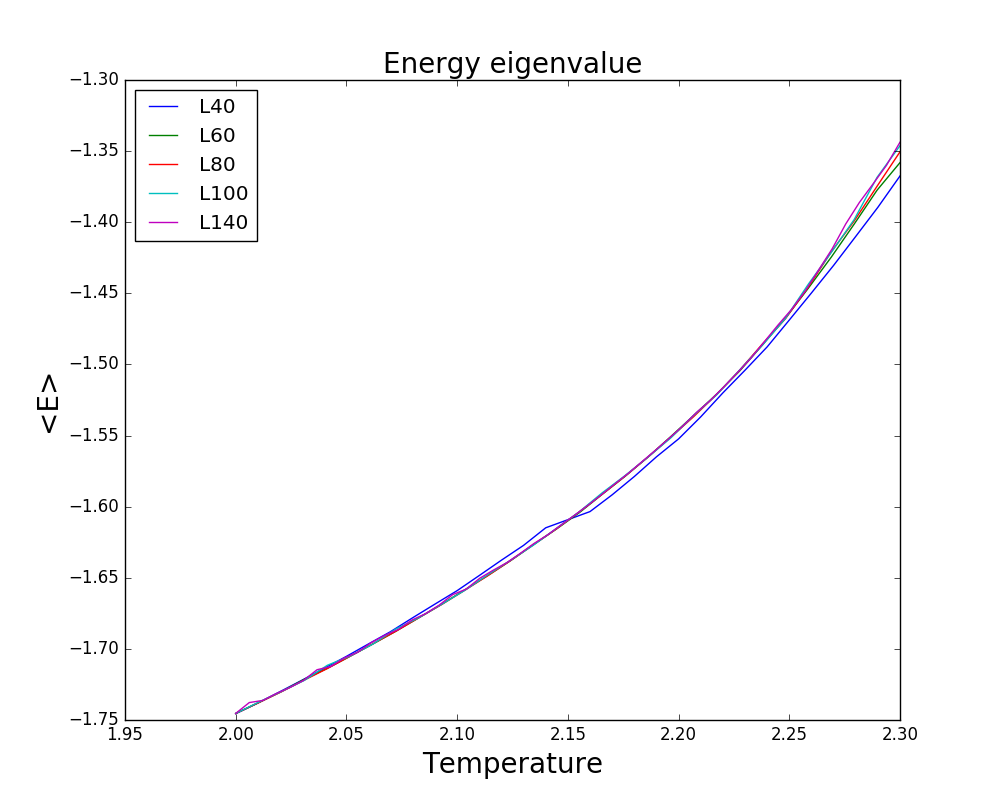
\includegraphics[scale=0.29]{../figures/task_e/energyeig.png}
\label{fig:cEeig}
\end{subfigure}
\begin{subfigure}{0.49 \textwidth}
\centering
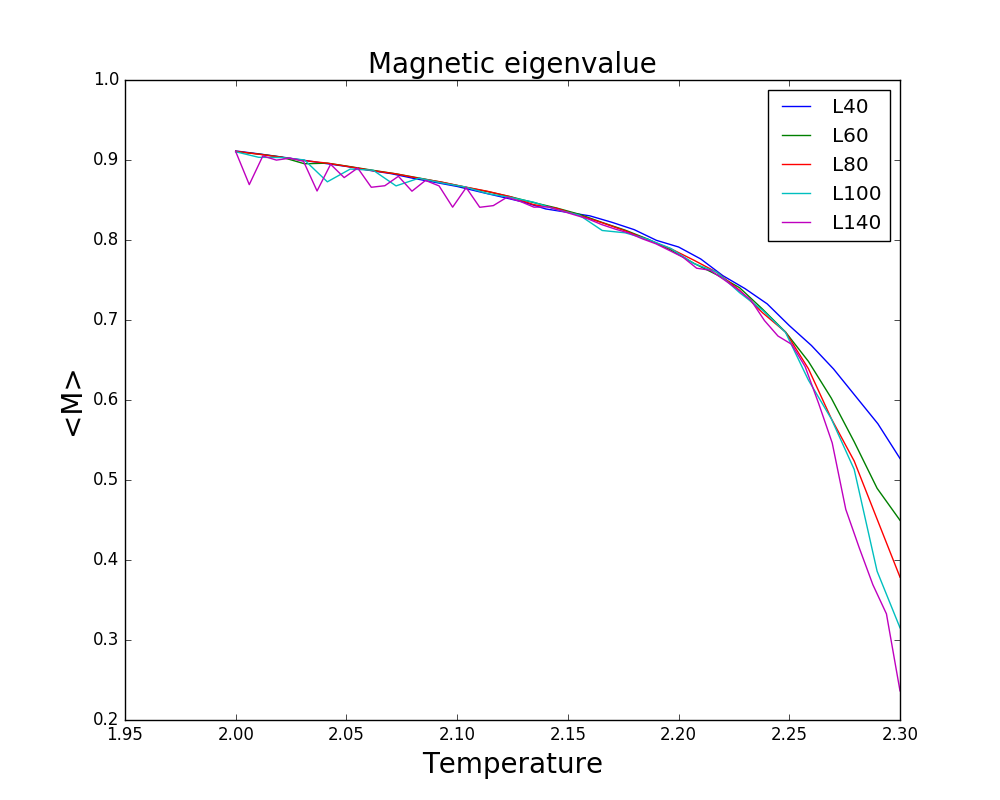
\includegraphics[scale=0.29]{../figures/task_e/Mageig.png}
\label{fig:cMeig} \\
\end{subfigure}
\begin{subfigure}{0.49 \textwidth}
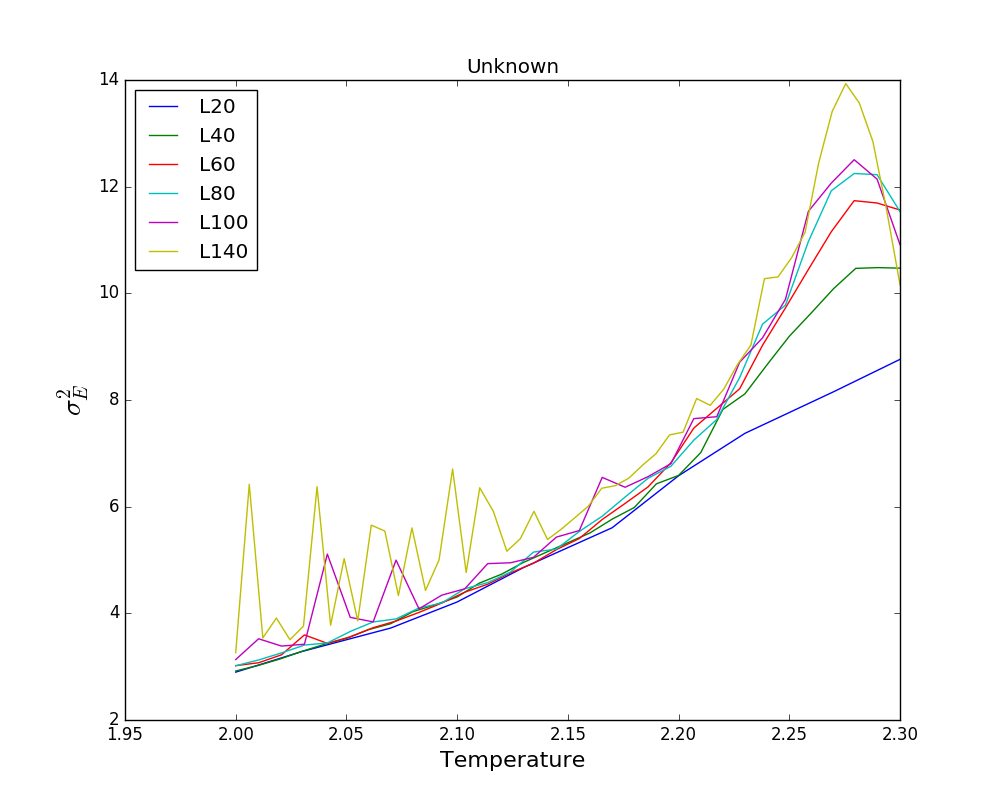
\includegraphics[scale=0.29]{../figures/task_e/sigmaE.png}
\label{fig:cEeig}
\end{subfigure}
\begin{subfigure}{0.49 \textwidth}
\centering
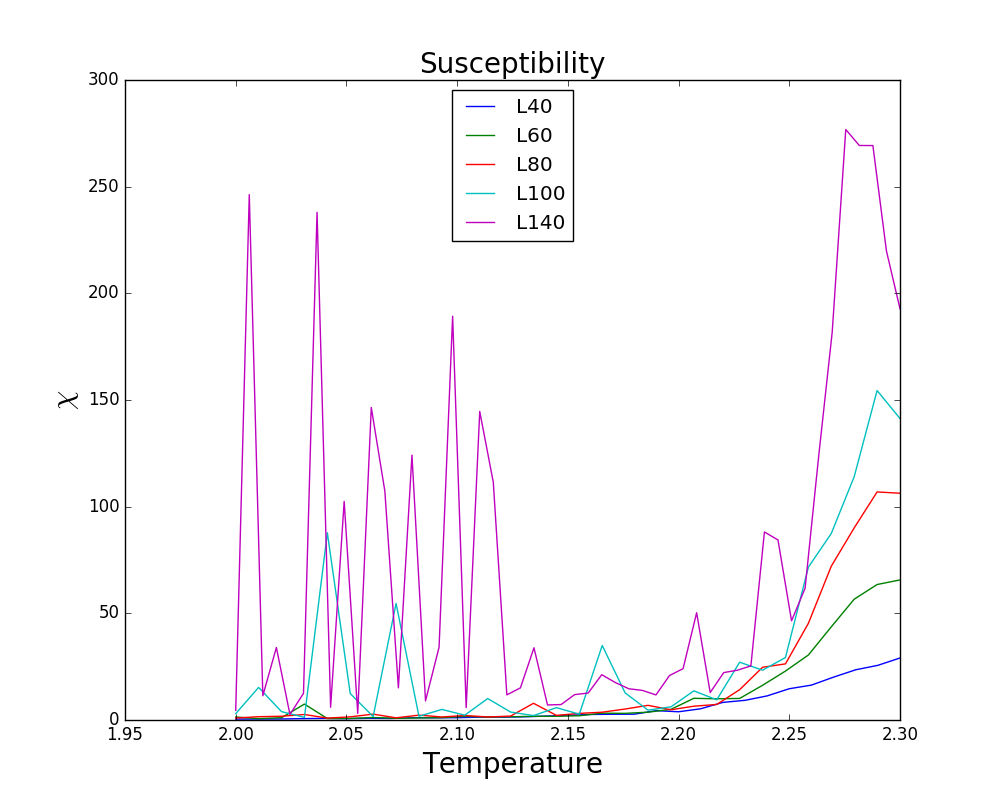
\includegraphics[scale=0.29]{../figures/task_e/suscept.png}
\label{fig:cMeig}
\end{subfigure}
\caption{Energy eigenvalues, magnetic eigenvalues, Heat capcity and Susceptibility as a function of different temperatures in the interal $T \in [2.0, 2,3]$ for different L-values. $dt = 0.1034$ for $L \in [40, 100]$ and $dt = 0.00612$ for L = 140. As we can see, there is a good deal unstability at L = 140.}
\label{fig:e}
\end{figure}
The phase shift will happen at the maximum value of $C_v$ and $\chi$. In table \ref{tab:e} the different max temperatures for $C_v$ and $\chi$ for each L is written down:
\begin{table}
\centering
\caption{Critical temperature for $C_v$ and $\chi$ as a function of L.}
\begin{tabular}{c|c|c}
L & $C_v$ & $\chi$ \\ \hline
40 & 2.28 & 2.3 \\
60 & 2.2793 & 2.3 \\
80 & 2.2793 & 2.2897 \\
100 & 2.2793 & 2.2897 \\
140 & 2.2755 & 2.2755 \\
\end{tabular}
\label{tab:e}
\end{table}
\subsection*{Discussion}
\subsubsection*{L = 2}
Looking at table \ref{tab:taskb} we can see that the values comes closer and closer to the analytical ones and then starts fluctuating around it with increasing Monte Carlo cycles. This is as we should expect given and I would deam this run stable at about 100000 Monte carlo Cycles. Comparing with our grafs in figure \ref{fig:c} this seems to be a reasonable assumption.
\subsubsection*{L = 20}
From figure \ref{fig:c} we can see that the values stabilizes at about 80 000 for T = 1.0 and 60 000 at T = 2.4. These values makes sense. When we start of the Monte Carlo cycles all spins are either randomly divided or all are pointing upwards. And as we see there is a big difference in the start before they close in on each other.  The reason why we have such a large threshold for T = 1.0 is maybe not clear. After all the y-axis on these plots are a lot shorter than for T = 2.4. It is simply because this was the point where the overall stability seemed to be from the graph. One could argue that since we don't have such a detailed graph of T = 2.4 we should have a lower threshold for T = 1.0 than we do for T = 2.4, but as we have 1000000 Monte Carlo cycles there is little harm done, and the graph is more stable at 80000 than at say, 30000.
\\ \\
Figure \ref{fig:cAcc} shows us that the number of accepted states increases rapidly with temperature. My theory is that since we only accpet $r \leq e^{-\beta \Delta E}$ in the metropolis and $\beta$ decreaces with larger T, this will make $e^{-\beta \Delta E}$ come closer to 1 for positive $\Delta E$. Therefore we will go faster towards equilibrium. Simply summarized: When we increase T, $\beta$ decreases and we have more accepted states. What is interesting to note is that we have the most rapid increase about around where the critical temperature found by Onsager is. \\ \\
The plots in fiugre \ref{fig:cProb} were a pain. I don't know where the problem is and after about 15 hours on this task alone I have given up and I am content with my results as they are. If I had done this project again I would have asked for help about this more than I did this time and wait until I was 100\% sure I had the correct answer. As we can see from the upper most plot, there are most energies around the start energy. This makes sense as we can see from figure \ref{fig:c} the cases of T = 1.0 are quickly becomming stable and there is little fluctiuation. \\
For T = 2.4 the energies are more spread out. Once again, this makes sense. First of all, there will be more accpeted states and as we see from figure \ref{fig:c} the values fluctuate more here than compared to the T = 1.0 case. \\
The variance values in table \ref{tab:var} are completely off and I think it has something to do with how we aquire our values. If I had done the task again, I would especially have focused on how I write to file and find out why the variance is weird while the plots make sense. \\
Another problem with the plots are that they are not correctly normalized. This is because I use the \texttt{.hist} function from \texttt{matplotlib.pyplot} and the normalize function there is not working for me.
\subsubsection*{L $\geq$ 20}
This was the most fun part of the program as we did huge calculations in a relatively short time period. As we can see from figure \ref{fig:e} the values are as eexpecting increasing with L and temperature with a peak in temperature at the critical temperature. From table \ref{tab:e} we can see that the critical temperatures comes closer and closer to the limit found by Onsager and this shows us that we have good data sets. \\
Why the L = 140 curve is acting out is a mystery to me, but I have two thoughts:
1. The algorithm becomes unstable for so large values of L. \\
2. Since we have more temperatures, there may be the same fluctuation in all graphs, but it is only here it shows. \\
I think the first point is the most likely. \\
Had I done the experiment again, I would have done this for even higher L and with the same temperatures for all L.
\\ \\
All timing was done by my friend who hasn't given me the data, but the last was done in right under two hours.
\subsection*{Conclusion}
This has been a fun project when one overlooks task d. We have found that there was a good correlation between the analytical and the numerical values. The algorithm becomes stable at around 100000 both for L = 2 and L = 20. Accepted states increases as temperature increases because $\beta = 1/T$. Our histograms in figure \ref{fig:cProb} are badly normalized, but make sense. The variance values found numerically with numpy are terribly wrong. \\

\bibliography{biblo}
\end{document}